\chapter{Afslutning}
\label{ch:afslutning}

% Fik vi opfyldt de overordnede produktkrav og vores egen
% kravspecifikation? Kom produktet til at virke? Hvis ikke hvad så? Og
% ellers som vi plejer med en konklusion...

% Vis billede af tux og logo

\mnote{Fælles}

\section{Mangler}

Vi nåede ikke at få lavet en kasse til at lukke elektronikken af,
hvilket dog heller ikke er så vigtigt.

Vi nåede ikke at få knaptrykket til at virke, så vi har ingen nødstop
eller restart knap. Det betyder også, at plotteren ikke har en
nulstillingsposition, men at nulstillingspositionen er det sted pennen
befinder sig, når plotningen påbegyndes.


\section{Delvis -- men dækkende -- implementering af HPGL}

Instruktionerne \texttt{PU}, \texttt{PD}, \texttt{PA}, \texttt{PR} og
\texttt{CI} er implementeret, og det er kun en lille del af hele
HPGL-formatet. Dog viser det sig tilsyneladende, at
\texttt{hpgl-distiller}\footnote{Se brugervejledningen
  side~\pageref{ch:brugervejledning}.} kun bruger instruktionerne
\texttt{PU}, \texttt{PD} og \texttt{PA}, så implementeringen er
dækkende til tegninger genereret af \texttt{hpgl-distiller}.


\section{Kvalitet af plottet}

I figur\vref{fig:plot-tux} ses Tux -- Linux-maskotten -- som
vektorgrafik og som plot i plotteren. Vektorbilledet er brugt til at
generere HPGL-billedet brugt til plottet. 


\begin{figure}[htbp]
  \centering
  \subfloat[Billede af Tux, fra \cite{bbt:tux-billede}.]{
    
\includegraphics[width=0.40\textwidth]{./img/Tux-simple}
  }
  \qquad
  \subfloat[Plot af billede.]{
    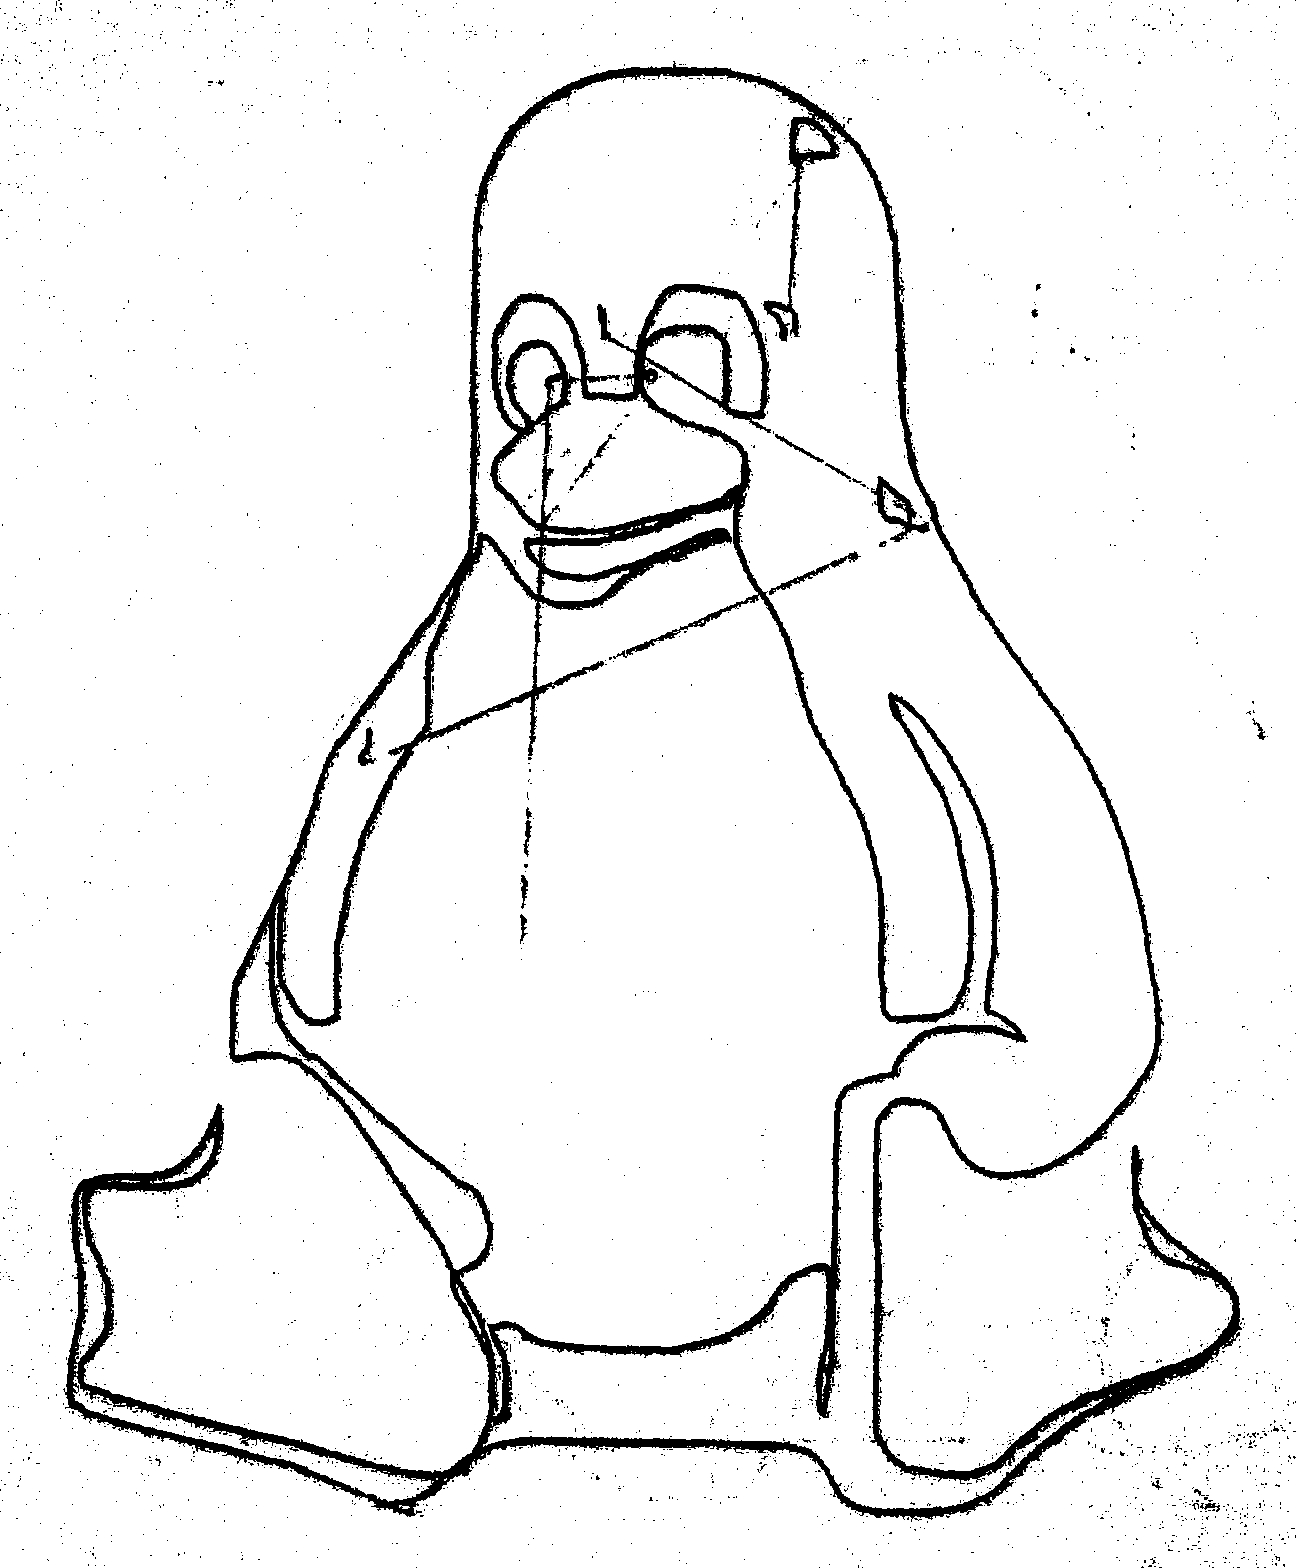
\includegraphics[width=0.40\textwidth]{./img/tux-plot}
  }
  \caption{Demonstration af kvaliteten af et plot.}
  \label{fig:plot-tux}
\end{figure}

Det er selvfølgelig op til hvert enkelt individ at vurdere kvaliteten,
men vi har lavet den bedømmelse, at resultatet er tilfredsstillende,
bortset fra enkelte småfejl såsom øjnenes placering og den
uforklarlige streng imellem kroppen.


\section{Motorproblemer}

Stepmotoren i $y$-aksen takker tilsyneladende over engang imellem,
hvilket resulterer i plots som i figur\vref{fig:plot-takker-over}.
Vi er kommet frem til at dette kan skyldes enten at stepmotoren er
for svag til at trække aksen stabilt eller at tandremmen er for stram.
Umiddelbart kan begge problemer løses relativt let ved enten erstating
af den nuværende stepmotor med en mere kraftig eller ved at løsne tandremmen.

\mnote{
  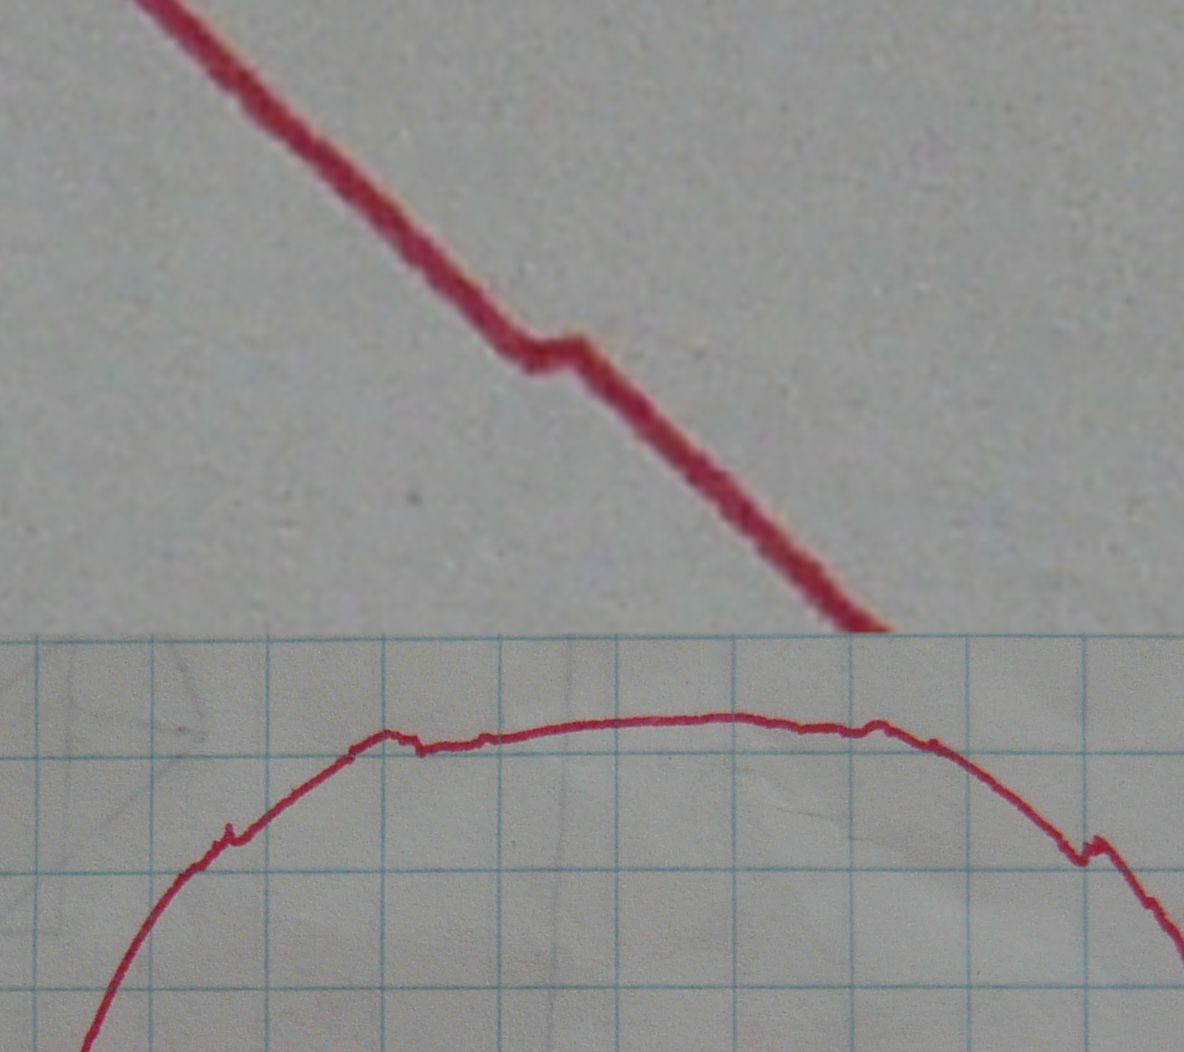
\includegraphics[width=\marginparwidth]{./img/takker-over}
  \captionof{figure}{Plot når $y$-motoren takker over}
  \label{fig:plot-takker-over}
}


%%% Local Variables: 
%%% mode: latex
%%% TeX-master: "../master"
%%% End: 